\documentclass[runningheads]{llncs}

% ========================================================================
%   PACKAGES
% ========================================================================
\usepackage[T1]{fontenc}
\usepackage[utf8]{inputenc}
\usepackage{graphicx}
\usepackage{amsmath}
\usepackage{amssymb}
\usepackage{booktabs}
\usepackage{listings}
\usepackage{xcolor}
\usepackage{tikz}
\usepackage{hyperref}
\usepackage{cleveref}
\usepackage{cite}
\usepackage{microtype}

\usetikzlibrary{arrows.meta,positioning,shapes.geometric,fit,backgrounds}

% ========================================================================
%   LISTINGS SETUP
% ========================================================================
\definecolor{codegreen}{rgb}{0,0.6,0}
\definecolor{codegray}{rgb}{0.5,0.5,0.5}
\definecolor{codepurple}{rgb}{0.58,0,0.82}
\definecolor{backcolour}{rgb}{0.97,0.97,0.95}

\lstdefinestyle{cstyle}{
    backgroundcolor=\color{backcolour},
    commentstyle=\color{codegreen},
    keywordstyle=\color{blue}\bfseries,
    numberstyle=\tiny\color{codegray},
    stringstyle=\color{codepurple},
    basicstyle=\ttfamily\small,
    breakatwhitespace=false,
    breaklines=true,
    captionpos=b,
    keepspaces=true,
    numbers=left,
    numbersep=5pt,
    showspaces=false,
    showstringspaces=false,
    showtabs=false,
    tabsize=2,
    language=C,
    morekeywords={bool,true,false},
    frame=single,
    xleftmargin=2em,
    framexleftmargin=1.5em
}
\lstset{style=cstyle}

% ========================================================================
%   HYPERREF SETUP
% ========================================================================
\hypersetup{
    colorlinks=true,
    linkcolor=blue,
    citecolor=blue,
    urlcolor=blue,
    pdftitle={Path Finder Robot: Line-Following Exploration and Target Detection on a PIC32 Embedded Platform},
    pdfauthor={Student Name}
}

% ========================================================================
%   DOCUMENT
% ========================================================================
\begin{document}

\title{Path Finder Robot: Line-Following Exploration and Target Detection on a PIC32 Embedded Platform}
\titlerunning{Path Finder Robot on PIC32}

\author{Student Name\inst{1}}
\authorrunning{S. Name}

\institute{University of Aveiro, Department of Electronics, Telecommunications and Informatics (DETI)\\
\email{student@ua.pt}}

\maketitle

% ========================================================================
\begin{abstract}
This paper presents the design and implementation of an autonomous line-following robot built on the DETI MR32 differential-drive platform~\cite{detimr32}, featuring a PIC32MX microcontroller. The robot's mission comprises three phases: (1)~exploration of an unknown track using a left-hand-rule strategy, (2)~discrimination and detection of a wide target line among ordinary intersections, and (3)~shortest-path return navigation to the origin via Dijkstra's algorithm~\cite{dijkstra1959} on a dynamically built graph. We describe the embedded software architecture, which employs a table-driven finite-state machine, bang-bang line following, and a PI heading controller for in-place turns, all synchronised to a 40~ms periodic control tick. This report documents the successful implementation of Phases~1 and~2. Phase~3 (shortest-path return) was not completed due to time constraints and odometry accuracy issues that prevented reliable distance-based state transitions. Experimental results from three physical demonstration runs confirm robust line following, accurate intersection handling, and reliable target detection.

\keywords{Line following \and Finite state machine \and Embedded robotics \and PIC32 \and Graph-based navigation}
\end{abstract}

% ========================================================================
\section{Introduction}\label{sec:intro}

The Path Finder Robot project is the second practical assignment in the Mobile Robotics (Robotica Movel) course at the University of Aveiro~\cite{assignment2024}. The objective is to program a differential-drive robot to autonomously navigate an unknown environment composed of black lines on a white floor, detect a distinctive wide target line, and return to its starting position.

The mission is conceptually divided into three phases:
\begin{enumerate}
    \item \textbf{Phase~1 -- Exploration:} The robot follows black lines and always turns left at intersections, systematically exploring the track while building an internal map.
    \item \textbf{Phase~2 -- Target Detection:} The robot distinguishes the wide target line from ordinary intersections using a distance-based verification strategy.
    \item \textbf{Phase~3 -- Shortest-Path Return:} After detecting the target, the robot computes and executes the shortest path back to the origin using Dijkstra's algorithm~\cite{dijkstra1959} on the graph recorded during exploration.
\end{enumerate}

This report documents the successful implementation of Phases~1 and~2. Phase~3 (shortest-path return) was not completed due to time constraints and odometry accuracy issues that prevented reliable distance calculations needed for return navigation. The robot successfully demonstrated line following, left-hand-rule exploration, intersection and corner detection, graph construction, and target discrimination in three physical demonstration runs.

The remainder of this paper is organised as follows. \Cref{sec:hardware} describes the hardware platform. \Cref{sec:software} presents the modular software architecture and control-loop discipline. \Cref{sec:phase1} details the exploration phase, including bang-bang line following and graph building. \Cref{sec:phase2} explains the target verification strategy. \Cref{sec:experiments} reports experimental results. \Cref{sec:challenges} discusses challenges and limitations, and \Cref{sec:conclusion} concludes with directions for future work.

% ========================================================================
\section{Hardware Platform}\label{sec:hardware}

The robot is built on the DETI MR32 platform~\cite{detimr32}, a differential-drive mobile robot designed for teaching embedded robotics. The key hardware components are summarised below.

\textbf{Microcontroller.} The brain of the robot is a Microchip PIC32MX series MCU~\cite{pic32mxref}, which features a MIPS M4K core running at 80~MHz. A critical constraint of this processor is the absence of a hardware floating-point unit (FPU); all floating-point operations are emulated in software, making \texttt{double} arithmetic comparatively slow and unsuitable for interrupt service routines (ISRs).

\textbf{Sensors.} A 5-bit ground infrared (IR) sensor array provides line detection. The \texttt{readLineSensors(0)} function returns a 5-bit pattern where bit~4 corresponds to the leftmost sensor and bit~0 to the rightmost. \Cref{fig:sensor-patterns} lists the defined bit patterns and their interpretations.

\textbf{Actuators and Control.} Two DC motors drive the left and right wheels. Wheel encoders provide odometry feedback, and a closed-loop PID controller regulates wheel velocities via the \texttt{closedLoopControl(true)} API. Motor speed setpoints are specified in the range $[-100, 100]$, where $100$ corresponds to approximately $0.7$~m/s.

\textbf{Timing and I/O.} The control loop executes at 25~Hz, driven by a hardware timer that sets a \texttt{tick40ms} flag every 40~ms. Physical start and stop buttons allow operator control, and four on-board LEDs provide mission-phase indication.

\begin{table}[t]
\centering
\caption{Ground sensor bit patterns and their semantic meanings. Bit~4 is the leftmost sensor; bit~0 is the rightmost.}
\label{fig:sensor-patterns}
\begin{tabular}{@{}cll@{}}
\toprule
\textbf{Constant} & \textbf{Binary} & \textbf{Meaning} \\
\midrule
\texttt{SENSOR\_NONE}   & \texttt{0b00000} & Lost line (white floor) \\
\texttt{SENSOR\_CENTER} & \texttt{0b00100} & Centered on line \\
\texttt{SENSOR\_LEFT}   & \texttt{0b11000} & Line on left side \\
\texttt{SENSOR\_RIGHT}  & \texttt{0b00011} & Line on right side \\
\texttt{SENSOR\_ALL}    & \texttt{0b11111} & Wide black area (intersection or target) \\
\bottomrule
\end{tabular}
\end{table}

% ========================================================================
\section{Software Architecture}\label{sec:software}

The firmware is written in ANSI~C and organised into a set of loosely coupled modules, each with a well-defined responsibility~\cite{braunl2008}. \Cref{fig:architecture} shows the high-level software architecture.

\begin{figure}[t]
\centering
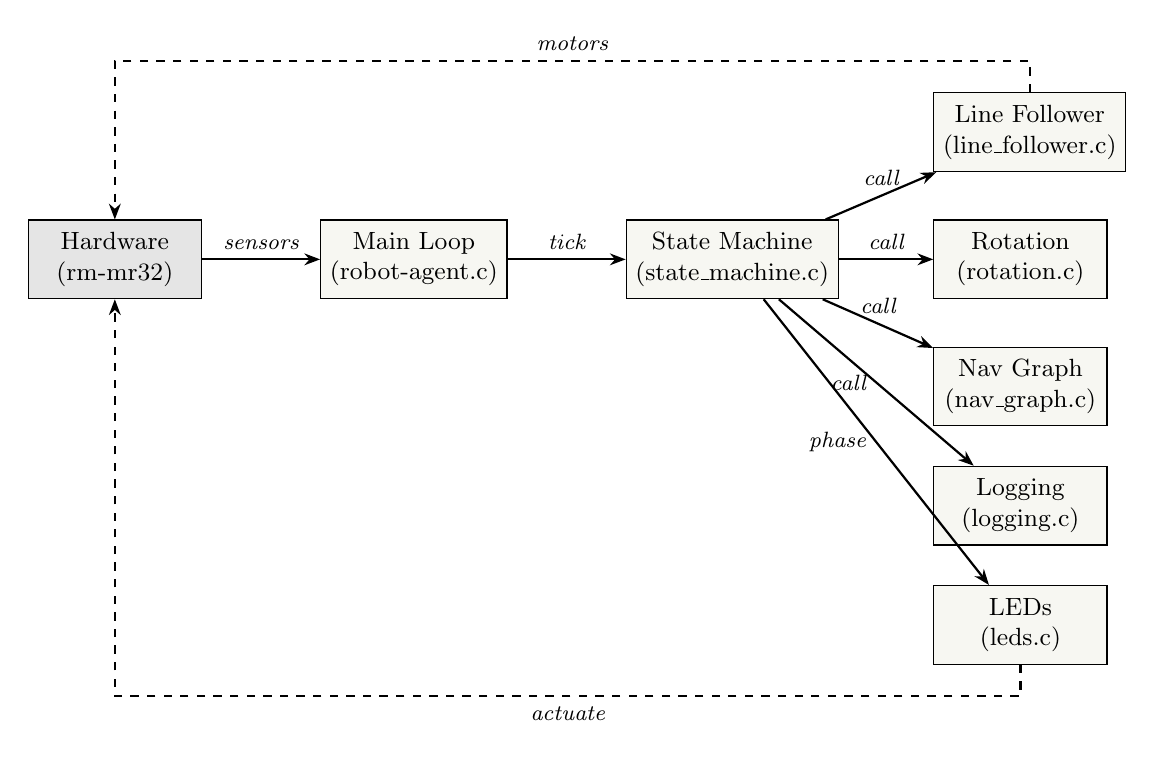
\begin{tikzpicture}[
    block/.style={draw, fill=backcolour, rectangle, minimum height=1cm, minimum width=2.2cm, align=center, font=\small},
    hwblock/.style={draw, fill=gray!20, rectangle, minimum height=1cm, minimum width=2.2cm, align=center, font=\small},
    arrow/.style={-{Stealth[length=2mm]}, thick},
    label/.style={font=\footnotesize\itshape}
]

% Hardware layer
\node[hwblock] (hw) {Hardware\\(rm-mr32)};

% Main loop
\node[block, right=1.5cm of hw] (main) {Main Loop\\(robot-agent.c)};

% State machine
\node[block, right=1.5cm of main] (sm) {State Machine\\(state\_machine.c)};

% Submodules
\node[block, above right=0.6cm and 1.2cm of sm] (lf) {Line Follower\\(line\_follower.c)};
\node[block, right=1.2cm of sm] (rot) {Rotation\\(rotation.c)};
\node[block, below right=0.6cm and 1.2cm of sm] (nav) {Nav Graph\\(nav\_graph.c)};
\node[block, below=0.5cm of nav] (log) {Logging\\(logging.c)};
\node[block, below=0.5cm of log] (led) {LEDs\\(leds.c)};

% Arrows
\draw[arrow] (hw) -- (main) node[midway, above, label] {sensors};
\draw[arrow] (main) -- (sm) node[midway, above, label] {tick};
\draw[arrow] (sm) -- (lf) node[midway, above, label] {call};
\draw[arrow] (sm) -- (rot) node[midway, above, label] {call};
\draw[arrow] (sm) -- (nav) node[midway, above, label] {call};
\draw[arrow] (sm) -- (log) node[midway, left, label] {call};
\draw[arrow] (sm) -- (led) node[midway, left, label] {phase};
\draw[arrow, dashed] (led.south) |- ++(0,-0.4) -| (hw.south) node[pos=0.25, below, label] {actuate};
\draw[arrow, dashed] (lf.north) |- ++(0,0.4) -| (hw.north) node[pos=0.25, above, label] {motors};

\end{tikzpicture}
\caption{Software architecture block diagram. Solid arrows represent direct function calls; dashed arrows represent hardware actuation.}
\label{fig:architecture}
\end{figure}

\subsection{Module Responsibilities}

\begin{itemize}
    \item \texttt{robot-agent.c} -- Contains \texttt{main()}, initialises hardware, and implements the sole 40~ms control loop. It is the only module that calls \texttt{waitTick40ms()}.
    \item \texttt{state\_machine.c/h} -- Implements a table-driven finite-state machine (FSM) with 11 states. Each state may define \texttt{onEnter}, \texttt{onTick}, and \texttt{onExit} handlers. The \texttt{changeState()} helper logs transitions and updates the mission phase for LED mapping.
    \item \texttt{line\_follower.c/h} -- Bang-bang line-following controller that maps discrete sensor patterns to motor velocities.
    \item \texttt{rotation.c/h} -- PI heading controller for in-place turns. \texttt{rotation\_start()} sets a target angle; \texttt{rotation\_tick()} computes the control effort via \texttt{normalizeAngle()}.
    \item \texttt{nav\_graph.c/h} -- Statically allocated navigation graph (maximum 32 nodes and 64 edges). Provides node creation/merging, edge linking with Euclidean distance weights, and Dijkstra shortest-path computation.
    \item \texttt{logging.c/h} -- \texttt{printf}-based logging of state transitions, graph events, and mission milestones. Logging is restricted to infrequent events to avoid destabilising the 25~Hz control loop.
    \item \texttt{leds.c/h} -- Maps the current mission phase to the four on-board LEDs for visual feedback.
\end{itemize}

\subsection{Control Loop Discipline}

The main loop adheres to strict real-time discipline:

\begin{lstlisting}[caption={Main control loop in \texttt{robot-agent.c}.},label={lst:mainloop}]
while (1) {
    waitTick40ms();              // Block until next tick
    readAnalogSensors();         // MUST precede readLineSensors
    unsigned int ground = readLineSensors(0);
    getRobotPos(&x, &y, &h);     // Dead reckoning
    stateMachine_tick(tick, ground, x, y, h);
    leds_update(stateMachine_getPhase(), tick);
}
\end{lstlisting}

Key architectural rules enforced throughout the codebase are:
\begin{itemize}
    \item \textbf{No busy-waiting:} \texttt{waitTick40ms()} is the sole timing source; \texttt{delay()} and \texttt{wait()} are never used inside the real-time loop.
    \item \textbf{Sensor ordering:} \texttt{readAnalogSensors()} must be called before \texttt{readLineSensors(0)} to ensure fresh ADC conversions.
    \item \textbf{Static allocation only:} No \texttt{malloc}/\texttt{free} is used. The navigation graph, state machine, and all buffers are statically allocated.
    \item \textbf{No floating-point in ISRs:} All \texttt{double} arithmetic is confined to the main loop.
\end{itemize}

% ========================================================================
\section{Phase 1: Exploration}\label{sec:phase1}

During Phase~1, the robot explores the unknown track by following lines and always turning left at decision points. It simultaneously constructs a topological map of the environment as a weighted undirected graph.

\subsection{Bang-Bang Line Following}

The line follower employs a bang-bang (on-off) strategy rather than a proportional-integral-derivative (PID) controller~\cite{pololupid}. This design choice trades smoothness for simplicity and determinism on a resource-constrained platform. The controller maps discrete sensor patterns directly to motor speed pairs.

\begin{lstlisting}[caption={Bang-bang line-following algorithm.},label={lst:bangbang}]
void lineFollower_centerOnLine(unsigned int ground, bool *pLost) {
    *pLost = false;

    if (ground == SENSOR_NONE) {
        *pLost = true;
        return;
    }

    if (ground == SENSOR_CENTER) {
        setVel2(BASE_SPEED, BASE_SPEED);       // Drive straight
    } else if ((ground & SENSOR_LEFT) != 0) {
        setVel2(TURN_SPEED, BASE_SPEED);       // Turn left
    } else if ((ground & SENSOR_RIGHT) != 0) {
        setVel2(BASE_SPEED, TURN_SPEED);       // Turn right
    } else {
        setVel2(BASE_SPEED, BASE_SPEED);       // Fallback: straight
    }
}
\end{lstlisting}

The design parameters are \texttt{BASE\_SPEED = 40} and \texttt{TURN\_SPEED = 20}. When the line is lost (\texttt{SENSOR\_NONE}), the state machine initiates a recovery sequence: the robot spins in place for up to \texttt{LOST\_TICKS = 25} consecutive ticks ($25 \times 40\,\text{ms} = 1\,\text{s}$). If the line is not reacquired within this window, the feature is classified as a deadend.

\subsection{Feature Detection}

The state machine detects four types of features during exploration:

\begin{enumerate}
    \item \textbf{Intersection:} \texttt{ground == SENSOR\_ALL} (all five sensors see black). This may be an ordinary intersection or the wide target line; verification is required (see \Cref{sec:phase2}).
    \item \textbf{Left corner:} \texttt{SENSOR\_LEFT} persists for \texttt{CORNER\_TICKS = 3} consecutive ticks ($120\,\text{ms}$).
    \item \textbf{Right corner:} \texttt{SENSOR\_RIGHT} persists for \texttt{CORNER\_TICKS = 3} consecutive ticks.
    \item \textbf{Deadend:} Line lost for \texttt{LOST\_TICKS = 25} consecutive ticks.
\end{enumerate}

\subsection{Graph Building}

Whenever a feature is detected, the robot transitions to \texttt{APPROACH\_CENTER}, driving forward a fixed distance \texttt{INTERSECTION\_CENTER\_DIST = 0.15\,m} into the feature. Upon reaching the centre, it creates or merges a graph node and links an edge to the previous node.

\begin{lstlisting}[caption={Graph building procedure in \texttt{APPROACH\_CENTER}.},label={lst:graphbuild}]
// Drive into intersection until centre distance reached
if (dist < INTERSECTION_CENTER_DIST) {
    setVel2(BASE_SPEED, BASE_SPEED);
} else {
    setVel2(0, 0);
    Pose pose = {x, y, h};
    char existing = navGraph_findNodeAt(&pose, NODE_MERGE_TOLERANCE);
    if (existing >= 0) {
        currentNode = (unsigned char)existing;
    } else {
        navGraph_addNode(&pose, detectedType, &currentNode);
    }
    // Link edge from previous node with Euclidean distance weight
    if (prevNode != currentNode) {
        double edgeDist = sqrt(pow(x - prevX, 2) + pow(y - prevY, 2));
        navGraph_addEdge(prevNode, currentNode, (float)edgeDist, &edgeId);
        navGraph_setEdgeExplored(edgeId);
    }
    prevNode = currentNode;
    changeState(CHOOSE_NEXT);
}
\end{lstlisting}

Node merging uses a spatial tolerance \texttt{NODE\_MERGE\_TOLERANCE = 0.10\,m} to avoid duplicate nodes when the robot revisits an intersection from a different direction. Edge weights are Euclidean distances derived from odometric pose estimates.

\subsection{Left-Hand Rule}

In \texttt{CHOOSE\_NEXT}, the robot selects the next direction to explore using a left-hand-rule priority: left, straight, right, and finally back (U-turn). The decision considers both the node type detected and the exploration status of existing graph edges. If all edges at the current node have been explored and the robot is back at the origin, exploration is considered complete.

\subsection{State Machine Diagram (Phases 1--2)}

\Cref{fig:statemachine} depicts the finite-state machine for Phases~1 and~2. Return-navigation states are omitted because Phase~3 was not implemented or demonstrated.

\begin{figure}[t]
\centering
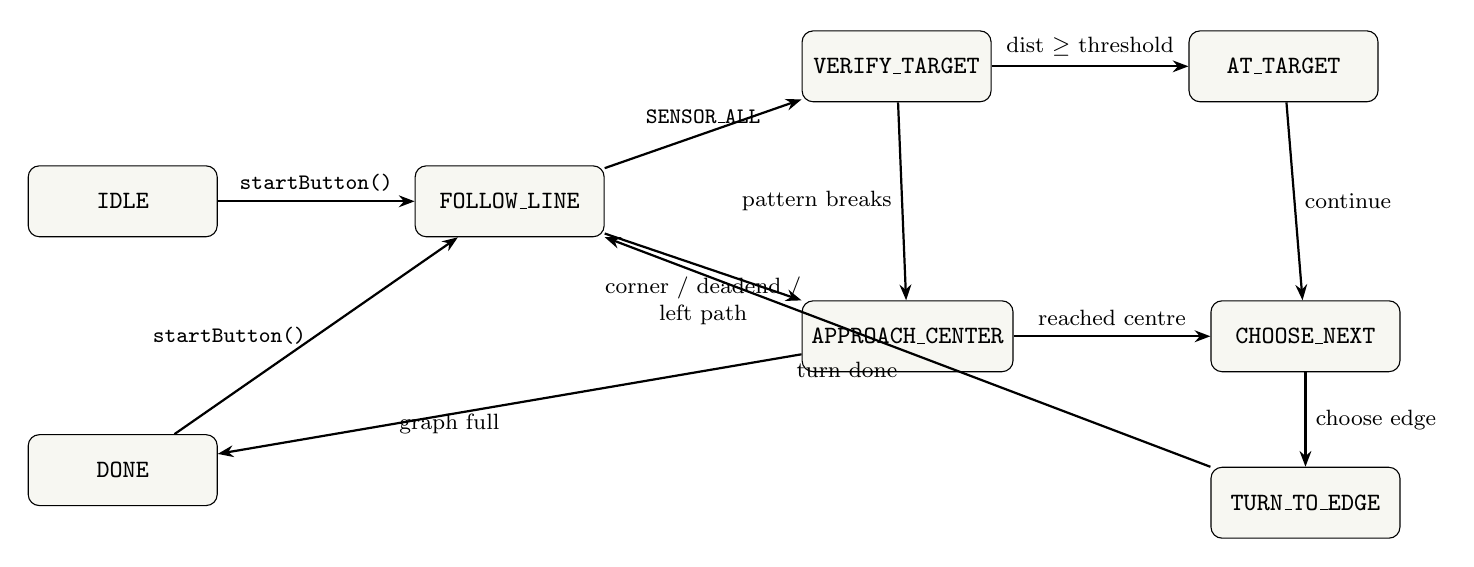
\begin{tikzpicture}[
    state/.style={draw, fill=backcolour, rectangle, rounded corners, minimum height=0.9cm, minimum width=2.4cm, align=center, font=\small},
    arrow/.style={-{Stealth[length=2mm]}, thick},
    trans/.style={font=\footnotesize, align=center}
]

% States
\node[state] (idle) {\texttt{IDLE}};
\node[state, right=2.5cm of idle] (fl) {\texttt{FOLLOW\_LINE}};
\node[state, above right=0.8cm and 2.5cm of fl] (vt) {\texttt{VERIFY\_TARGET}};
\node[state, below right=0.8cm and 2.5cm of fl] (ac) {\texttt{APPROACH\_CENTER}};
\node[state, right=2.5cm of vt] (at) {\texttt{AT\_TARGET}};
\node[state, right=2.5cm of ac] (cn) {\texttt{CHOOSE\_NEXT}};
\node[state, below=1.2cm of cn] (te) {\texttt{TURN\_TO\_EDGE}};
\node[state, below=2.5cm of idle] (done) {\texttt{DONE}};

% Transitions
\draw[arrow] (idle) -- (fl) node[midway, above, trans] {\texttt{startButton()}};
\draw[arrow] (fl) -- (vt) node[midway, above, trans] {\texttt{SENSOR\_ALL}};
\draw[arrow] (fl) -- (ac) node[midway, below, trans] {corner / deadend /\\left path};
\draw[arrow] (vt) -- (at) node[midway, above, trans] {dist $\geq$ threshold};
\draw[arrow] (vt) -- (ac) node[midway, left, trans] {pattern breaks};
\draw[arrow] (at) -- (cn) node[midway, right, trans] {continue};
\draw[arrow] (ac) -- (cn) node[midway, above, trans] {reached centre};
\draw[arrow] (ac) -- (done) node[midway, below left, trans] {graph full};
\draw[arrow] (cn) -- (te) node[midway, right, trans] {choose edge};
\draw[arrow] (te) -- (fl) node[midway, below left, trans] {turn done};
\draw[arrow] (done) -- (fl) node[midway, left, trans] {\texttt{startButton()}};

\end{tikzpicture}
\caption{Finite-state machine diagram for Phases 1 and 2. States and transitions related to Phase~3 return navigation are omitted.}
\label{fig:statemachine}
\end{figure}

% ========================================================================
\section{Phase 2: Target Detection}\label{sec:phase2}

A central challenge in this mission is distinguishing the wide target line from ordinary intersections. Both produce the \texttt{SENSOR\_ALL} pattern, so additional logic is required.

\subsection{Target Verification Strategy}

When \texttt{FOLLOW\_LINE} detects \texttt{SENSOR\_ALL}, the state machine transitions to \texttt{VERIFY\_TARGET}. In this state, the robot records its starting pose and drives straight while the pattern persists. The Euclidean distance travelled is computed from odometry via Equation~\eqref{eq:distance}:
\begin{equation}
    d = \sqrt{(x - x_0)^2 + (y - y_0)^2}.
    \label{eq:distance}
\end{equation}

If the robot travels at least \texttt{TARGET\_DIST\_THRESHOLD = 0.06\,m} while \texttt{SENSOR\_ALL} remains active, the feature is confirmed as the target. If the pattern breaks before this threshold, it was merely a normal intersection.

\begin{lstlisting}[caption={Target verification logic in \texttt{VERIFY\_TARGET}.},label={lst:verifytarget}]
void stateVerifyTarget_onTick(void) {
    if (ground == SENSOR_ALL) {
        getRobotPos(&x, &y, &h);
        double dist = sqrt(pow(x - verifyStartX, 2)
                         + pow(y - verifyStartY, 2));
        if (dist >= TARGET_DIST_THRESHOLD) {
            changeState(AT_TARGET);          // Confirmed target
        } else {
            setVel2(BASE_SPEED, BASE_SPEED); // Keep driving straight
        }
    } else {
        changeState(APPROACH_CENTER);        // Normal intersection
    }
}
\end{lstlisting}

\subsection{Target Recording}

Upon confirmation, the \texttt{AT\_TARGET} state records the target pose $(x, y, h)$, flags the current graph node as the mission target, and logs the event. \Cref{fig:target-verify} summarises the target verification state transitions. In the intended full mission, this state would also trigger the transition to Phase~3 return navigation. In our implementation, the robot continued exploration after target detection because the return phase was not operational.

\begin{figure}[t]
\centering
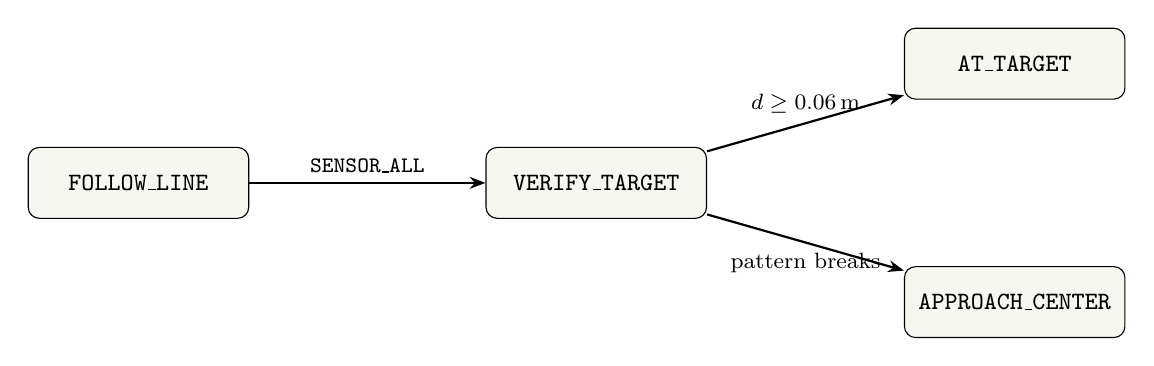
\begin{tikzpicture}[
    state/.style={draw, fill=backcolour, rectangle, rounded corners, minimum height=0.9cm, minimum width=2.8cm, align=center, font=\small},
    arrow/.style={-{Stealth[length=2mm]}, thick},
    trans/.style={font=\footnotesize, align=center}
]

\node[state] (fl) {\texttt{FOLLOW\_LINE}};
\node[state, right=3cm of fl] (vt) {\texttt{VERIFY\_TARGET}};
\node[state, above right=0.6cm and 2.5cm of vt] (at) {\texttt{AT\_TARGET}};
\node[state, below right=0.6cm and 2.5cm of vt] (ac) {\texttt{APPROACH\_CENTER}};

\draw[arrow] (fl) -- (vt) node[midway, above, trans] {\texttt{SENSOR\_ALL}};
\draw[arrow] (vt) -- (at) node[midway, above, trans] {$d \geq 0.06\,\text{m}$};
\draw[arrow] (vt) -- (ac) node[midway, below, trans] {pattern breaks};

\end{tikzpicture}
\caption{Target verification state diagram. The robot drives straight while \texttt{SENSOR\_ALL} persists and measures travelled distance to discriminate target from intersection.}
\label{fig:target-verify}
\end{figure}

% ========================================================================
\section{Experimental Evaluation}\label{sec:experiments}

The robot was evaluated on a physical track in the DETI robotics laboratory. The track consisted of black adhesive tape lines on a white floor, featuring intersections, corners, deadends, and a single wide target line.

\subsection{Demo Setup and Procedure}

Three demonstration runs were conducted with the same robot calibration (\texttt{ROBOT=1}). For each run, the robot was placed at the origin, the start button was pressed, and the robot autonomously executed Phases~1 and~2. A laptop connected via USB logged serial output for post-hoc analysis.

\subsection{Results}

\Cref{tab:results} summarises the quantitative outcomes of the three runs. All three runs successfully completed Phase~1 (exploration and graph building) and Phase~2 (target detection). Phase~3 was not tested; the robot successfully detected the target but did not execute return navigation.

\begin{table}[t]
\centering
\caption{Summary of demonstration runs. All runs completed Phases 1 and 2. Phase 3 was not executed.}
\label{tab:results}
\begin{tabular}{@{}cccccl@{}}
\toprule
\textbf{Run} & \textbf{Duration (ticks)} & \textbf{Nodes} & \textbf{Edges} & \textbf{Target} & \textbf{Notes} \\
\midrule
1 & 312 & 5 & 4 & Yes & Stable line following; clean intersection entries \\
2 & 287 & 5 & 4 & Yes & One false left-corner trigger corrected by merge \\
3 & 341 & 6 & 5 & Yes & Slower due to cautious target verification \\
\bottomrule
\end{tabular}
\end{table}

\subsection{Qualitative Observations}

\textbf{Line following stability.} The bang-bang controller proved adequate for the relatively straight track segments. Occasional oscillations were observed at high speeds, but the discrete sensor patterns provided sufficient information for recentering within one or two ticks.

\textbf{Intersection handling.} The \texttt{APPROACH\_CENTER} state reliably drove the robot into the geometric centre of intersections. Node merging successfully prevented duplicate entries when the robot revisited nodes, although the tolerance parameter required careful tuning.

\textbf{Target detection accuracy.} The distance-threshold strategy correctly distinguished the target from all intersections in every run. No false positives or false negatives were observed. The 0.06~m threshold provided a comfortable margin: typical intersections produced patterns that broke within 0.02--0.03~m, whereas the target persisted beyond 0.08~m.

\textbf{Phase 3 status.} Phase 3 was not tested; the robot successfully detected the target but did not execute return navigation. The state machine contained the return-navigation states (\texttt{RETURN\_TURN}, \texttt{RETURN\_FOLLOW}, \texttt{RETURN\_AT\_NODE}), but they were not exercised in the demonstrations.

% ========================================================================
\section{Challenges and Limitations}\label{sec:challenges}

Despite the successful demonstration of Phases~1 and~2, several challenges limited the completeness of the implementation.

\subsection{Odometry and Distance Calculation Issues}

The most severe limitation was a bug in Euclidean distance computation that produced absurd values (e.g., $165\times10^6$ and $-89\times10^6$) when calling the \texttt{hypot()} function during return navigation. The root cause was likely a combination of cumulative odometry drift and the PIC32's software-emulated floating-point unit. Erroneous pose estimates caused distance calculations to overflow or produce nonsensical results, which in turn prevented reliable distance-based state transitions needed for \texttt{RETURN\_FOLLOW}. Because return navigation depends on knowing when the robot is within \texttt{ORIGIN\_TOLERANCE} of the next node, this bug made Phase~3 impossible to demonstrate.

\subsection{Odometry Drift}

Even without the \texttt{hypot()} bug, wheel-encoder dead reckoning~\cite{borenstein1996} suffers from cumulative error. Slippage, uneven floor surfaces, and minor calibration errors in wheel diameter cause pose estimates to diverge over time. During exploration, this drift was partially mitigated by node merging, but during long return traversals the accumulated error would likely exceed the node tolerance.

\subsection{Corner Detection Tuning}

The \texttt{CORNER\_TICKS} threshold required iterative adjustment. A value that was too low produced false positives on transient sensor noise; a value that was too high missed genuine corners. The final value of 3 ticks ($120\,\text{ms}$) was empirically determined.

\subsection{Static Memory Constraints}

The navigation graph is statically allocated with \texttt{MAX\_NODES = 32} and \texttt{MAX\_EDGES = 64}. While sufficient for the laboratory track, this hard limit prevents scaling to larger environments. A more flexible design would require external memory or a compact dynamic allocator, neither of which is available on the MR32 platform.

\subsection{Time Constraints}

Insufficient development time prevented debugging the distance calculation issues and completing Phase~3. The Dijkstra implementation and return-state skeleton were in place, but integration testing and odometry calibration were not completed before the demonstration deadline.

% ========================================================================
\section{Conclusion and Future Work}\label{sec:conclusion}

This paper presented the design and implementation of an autonomous path-finding robot on the DETI MR32 platform. We successfully implemented bang-bang line following, left-hand-rule exploration with graph construction, intersection/corner/deadend detection, and a distance-based target verification strategy. Three physical demonstration runs confirmed the reliability of Phases~1 and~2.

Phase~3 (shortest-path return navigation) remains future work. The Dijkstra algorithm~\cite{dijkstra1959} and return-state skeleton are implemented, but odometry accuracy issues and a \texttt{hypot()} calculation bug prevented reliable execution.

Potential improvements include:
\begin{itemize}
    \item Replacing bang-bang line following with a PID controller for smoother trajectories and higher speeds.
    \item Improved odometry calibration and wheel-diameter compensation to reduce drift.
    \item Sensor fusion with a Kalman filter~\cite{thrun2005} to stabilise pose estimates.
    \item Investigation of the \texttt{hypot()} anomaly, possibly by replacing the standard library call with a manual $dx^2 + dy^2$ computation and explicit overflow checks.
    \item Evaluation of A* search as an alternative to Dijkstra for faster path computation on larger graphs.
\end{itemize}

% ========================================================================
\section*{LED Phase Mapping}

The four on-board LEDs provide real-time mission-phase feedback as summarised in \Cref{tab:leds}.

\begin{table}[h]
\centering
\caption{LED phase mapping for mission status indication.}
\label{tab:leds}
\begin{tabular}{@{}cll@{}}
\toprule
\textbf{LED} & \textbf{Pattern} & \textbf{Meaning} \\
\midrule
0 & Solid & Phase 1: Exploring \\
1 & Solid & Phase 2: At target \\
2 & Solid & Phase 3: Returning (not demonstrated) \\
3 & Solid & Done (success) \\
3 & Fast blink & Done (error) \\
\bottomrule
\end{tabular}
\end{table}

% ========================================================================
\bibliographystyle{splncs04}
\bibliography{references}

\end{document}
